\section{Introduction}
Terahertz (THz) waves, situated in the electromagnetic spectrum between microwaves and infrared, span a frequency range of approximately 0.1 THz to 10 THz. They are utilized in various fields due to their unique properties. For instance, because THz waves can penetrate most non-metallic materials, they are beneficial in applications such as security scanning and non-destructive testing. Additionally, THz waves can capture information regarding the rotational and vibrational states of molecules, thus enabling their use in the detection and analysis of chemical substances; as well as the imaging of biological tissues.

Imaging across various electromagnetic wave bands, including X-rays and visible light, has revolutionized our daily lives. In medical diagnostics, X-ray imaging is crucial  for detecting conditions such as cancer and dental diseases, owing to its high penetration depth through various materials. Visible-light imaging has not only transformed the manner by which we record life but has also contributed to the development of artificial intelligence (AI) applications in surveillance security and surface-defect inspection. However, both of these imaging techniques have unresolved issues. Ionizing X-ray imaging can harm biological entities, thus severely limiting its application. Non-ionizing and non-destructive visible light imaging cannot probe the interiors of most optically opaque objects because of the highly absorptive and scattering behavior of light in the visible band.

THz imaging can be used to address these issues. THz imaging, which creates images by measuring the intensity or phase of THz waves, is non-ionizing and non-destructive and has garnered significant attention for its ability to classify materials as well as detect and inspect objects. Because THz radiation can partially penetrate various optically opaque materials, hidden information regarding the material is transmitted along with the wave, thus enabling the visualization of the interior without damaging the exterior~\cite{thz_imaging1,thz_imaging2,thz_imaging3,thz_imaging4}.

Over the recent decades, terahertz time-domain spectroscopy (THz-TDS) has become one of the most prominent forms of THz imaging; it enables non-invasive evaluations owing to its unique ability to extract the geometric and multifunctional information of objects. Because of its distinctive material interaction information in multi-dimensional domains such as space, time, frequency, and phase, THz-TDS imaging has been applied in various emerging areas, including drug detection~\cite{kawase2003nondest}, industrial inspection, cultural-heritage examination~\cite{fukunaga2016thz}, advanced-material investigation~\cite{spies2020terahertz}, and cancer detection~\cite{bowman2018pulsed}.

\begin{figure*}[htbp]
    \centering
    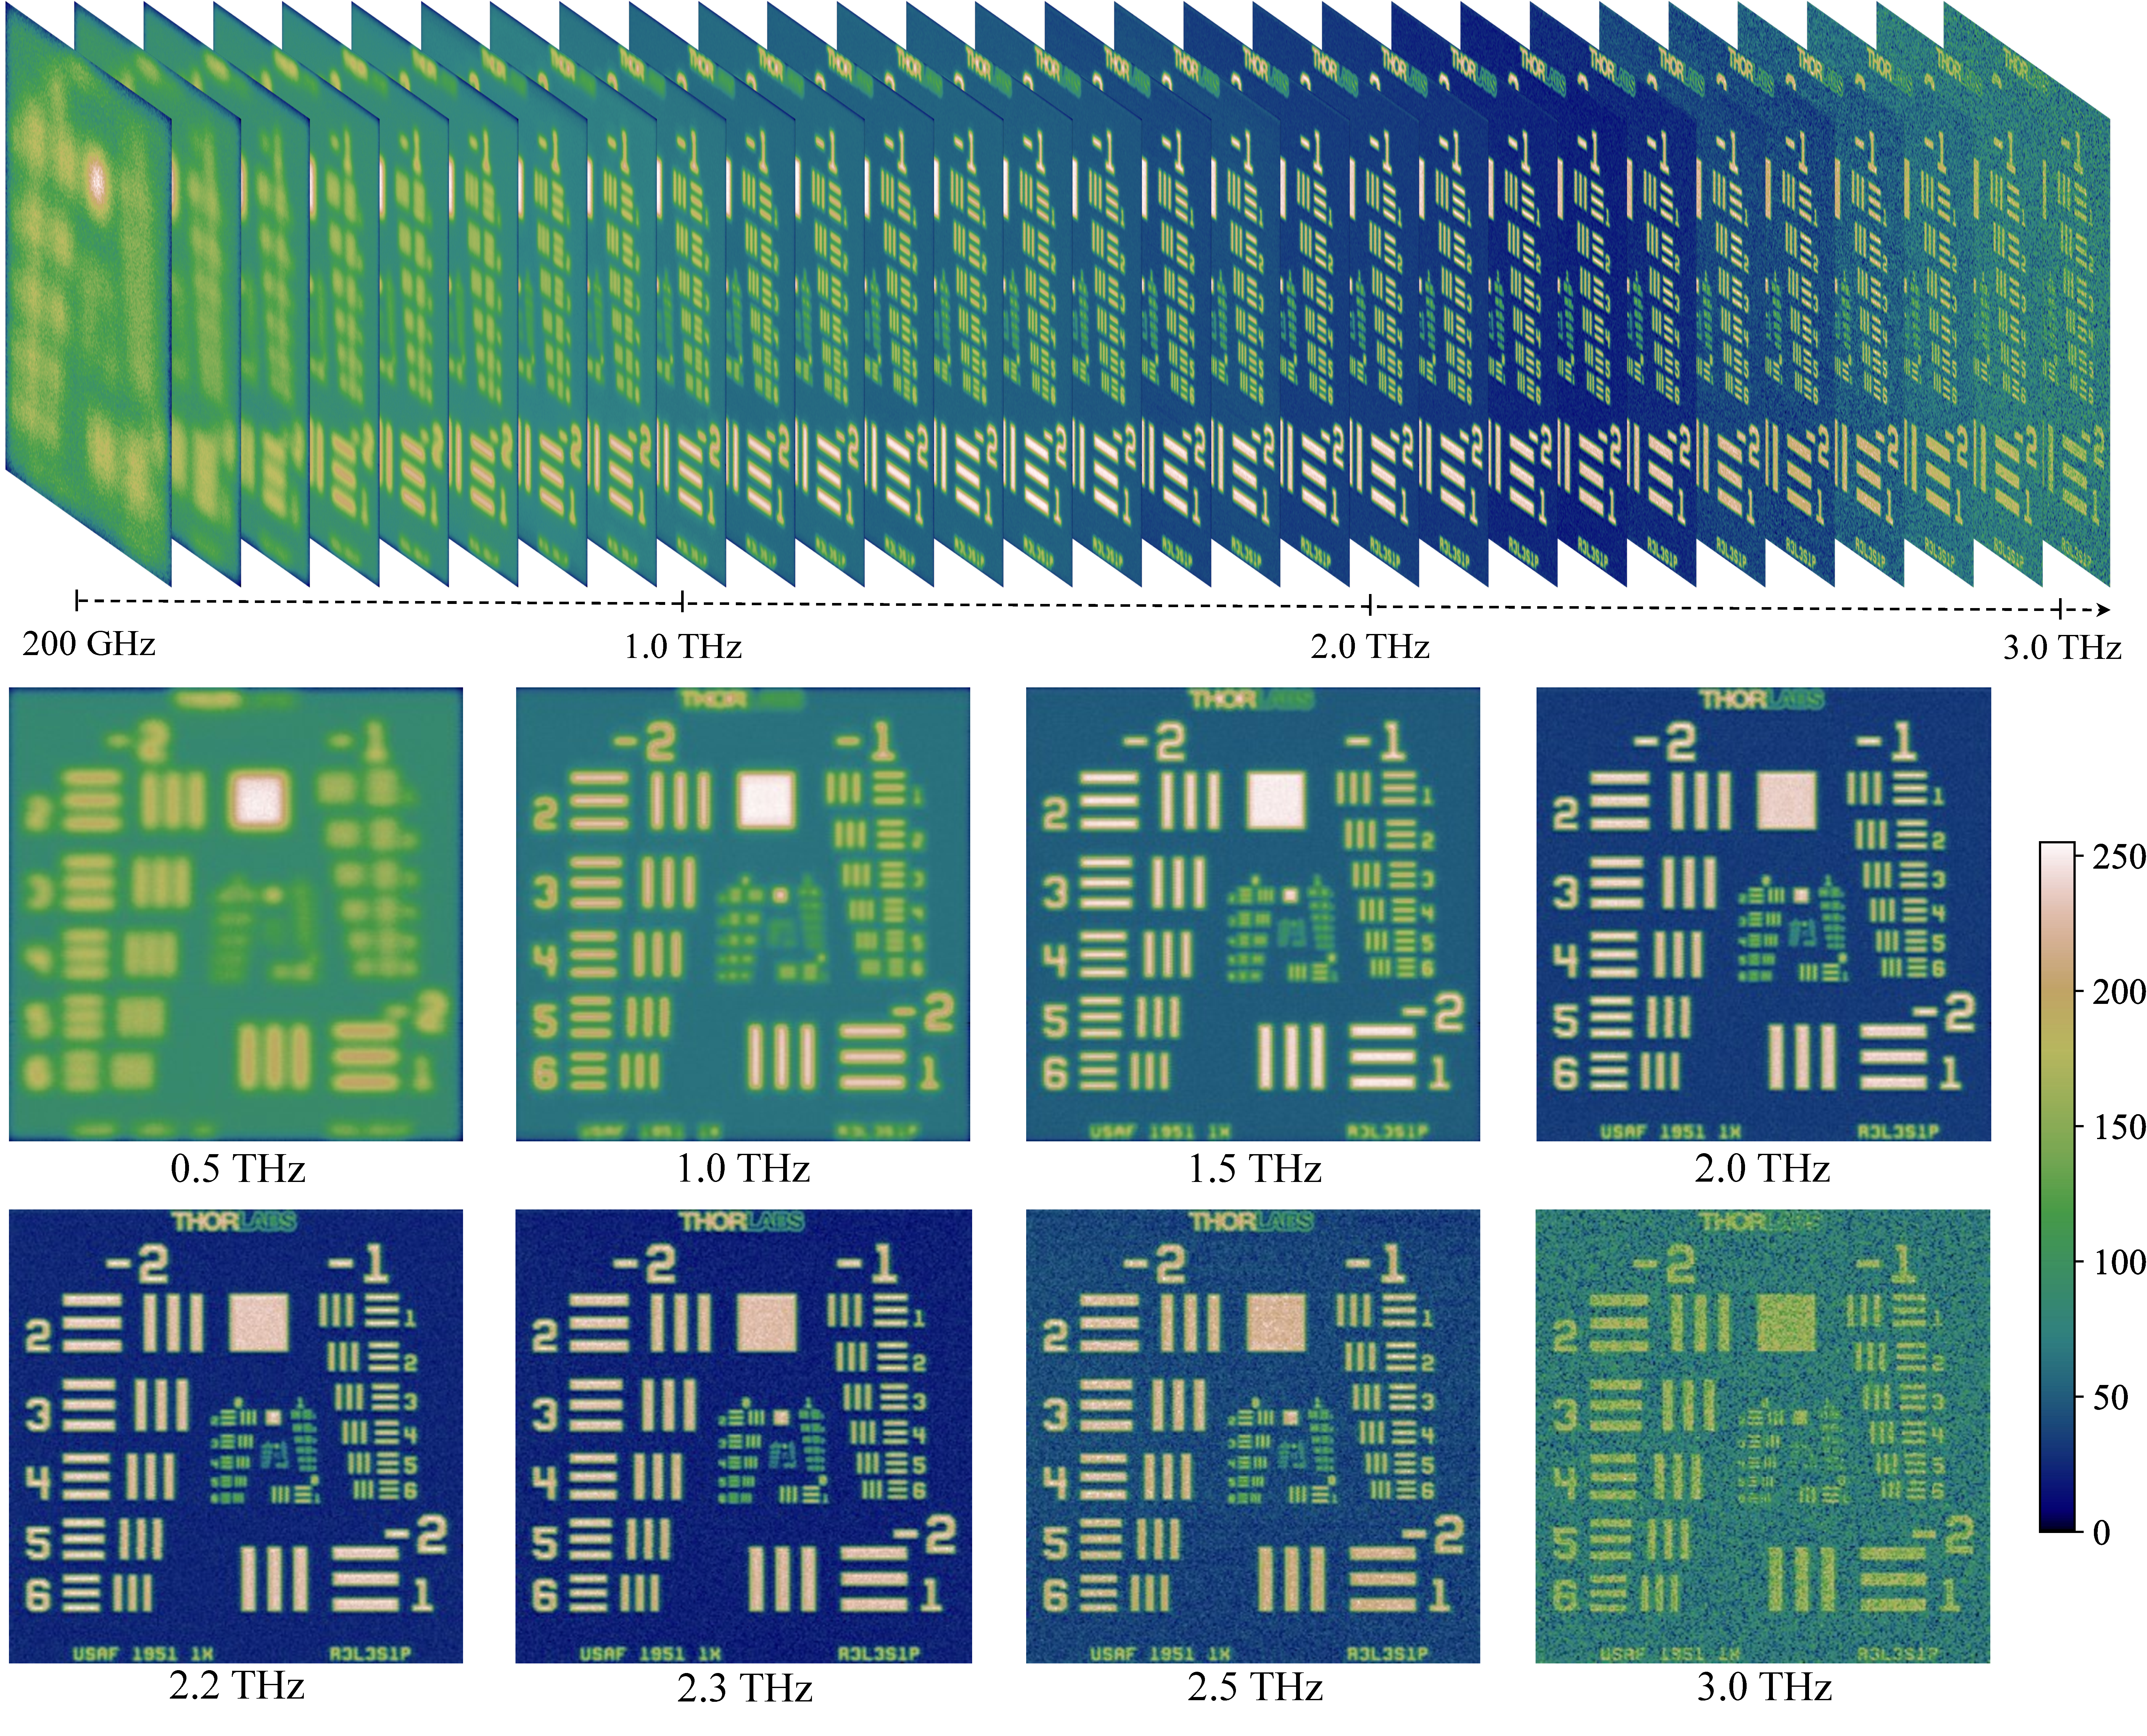
\includegraphics[width=0.85\textwidth]{fig/Ryu-fig1.pdf}
    \caption{THz SAHS image of the positive USAF 1951 resolution test target.}
    \label{fig:hyperspectral}
\end{figure*}

\IEEEpubidadjcol % 글자 겹치는거 방지용 
However, THz imaging is typically associated with image quality degradation owing to its strong water-absorption characteristics and low noise tolerance, thus resulting in undesirable blurring and distortion. Additionally, THz images obtained using THz-TDS system exhibit distinctly different characteristics depending on the frequency. Fig.~\ref{fig:hyperspectral} shows a THz self-aligned hyperspectral (SAHS) image obtained using the THz-TDS system of the positive United States Air Force (USAF) 1951 resolution test target (Thorlabs R3L3S1P). It shows frequency-specific images ranging from 200 GHz to 3 THz, in increments of 0.1 THz. Since the pixel values at the same location in SAHS images are acquired from the same TDS data, images of all frequencies within the SAHS image are automatically aligned without additional post-processing. All the THz images used in this study are based on the color map shown in Fig.~\ref{fig:hyperspectral}. Images in the lower-frequency band appear visually blurred but less noisy owing to the diffraction limit, whereas those in the higher frequencies offer better spatial resolution but increased noise owing to a lower signal-to-noise ratio (SNR).

Fig.~\ref{fig:iqa} shows the variations in the image sharpness, noise level, and contrast with frequency. The x-axis represents frequency, the left y-axis indicates the sharpness and noise level~\cite{chen2015noiselevel}, and the right y-axis represents the contrast. The image contrast increases gradually with frequency and reaches a maximum at 2.2 THz before decreasing. The sharpness increases continually with frequency, whereas the noise level decreases up to 1.0 THz and then increase as the frequency increase. The detailed descriptions of each image quality assessment metric are provided in Appendix~\ref{subsec:iqa}.

\begin{figure}[htbp]
    \centering
    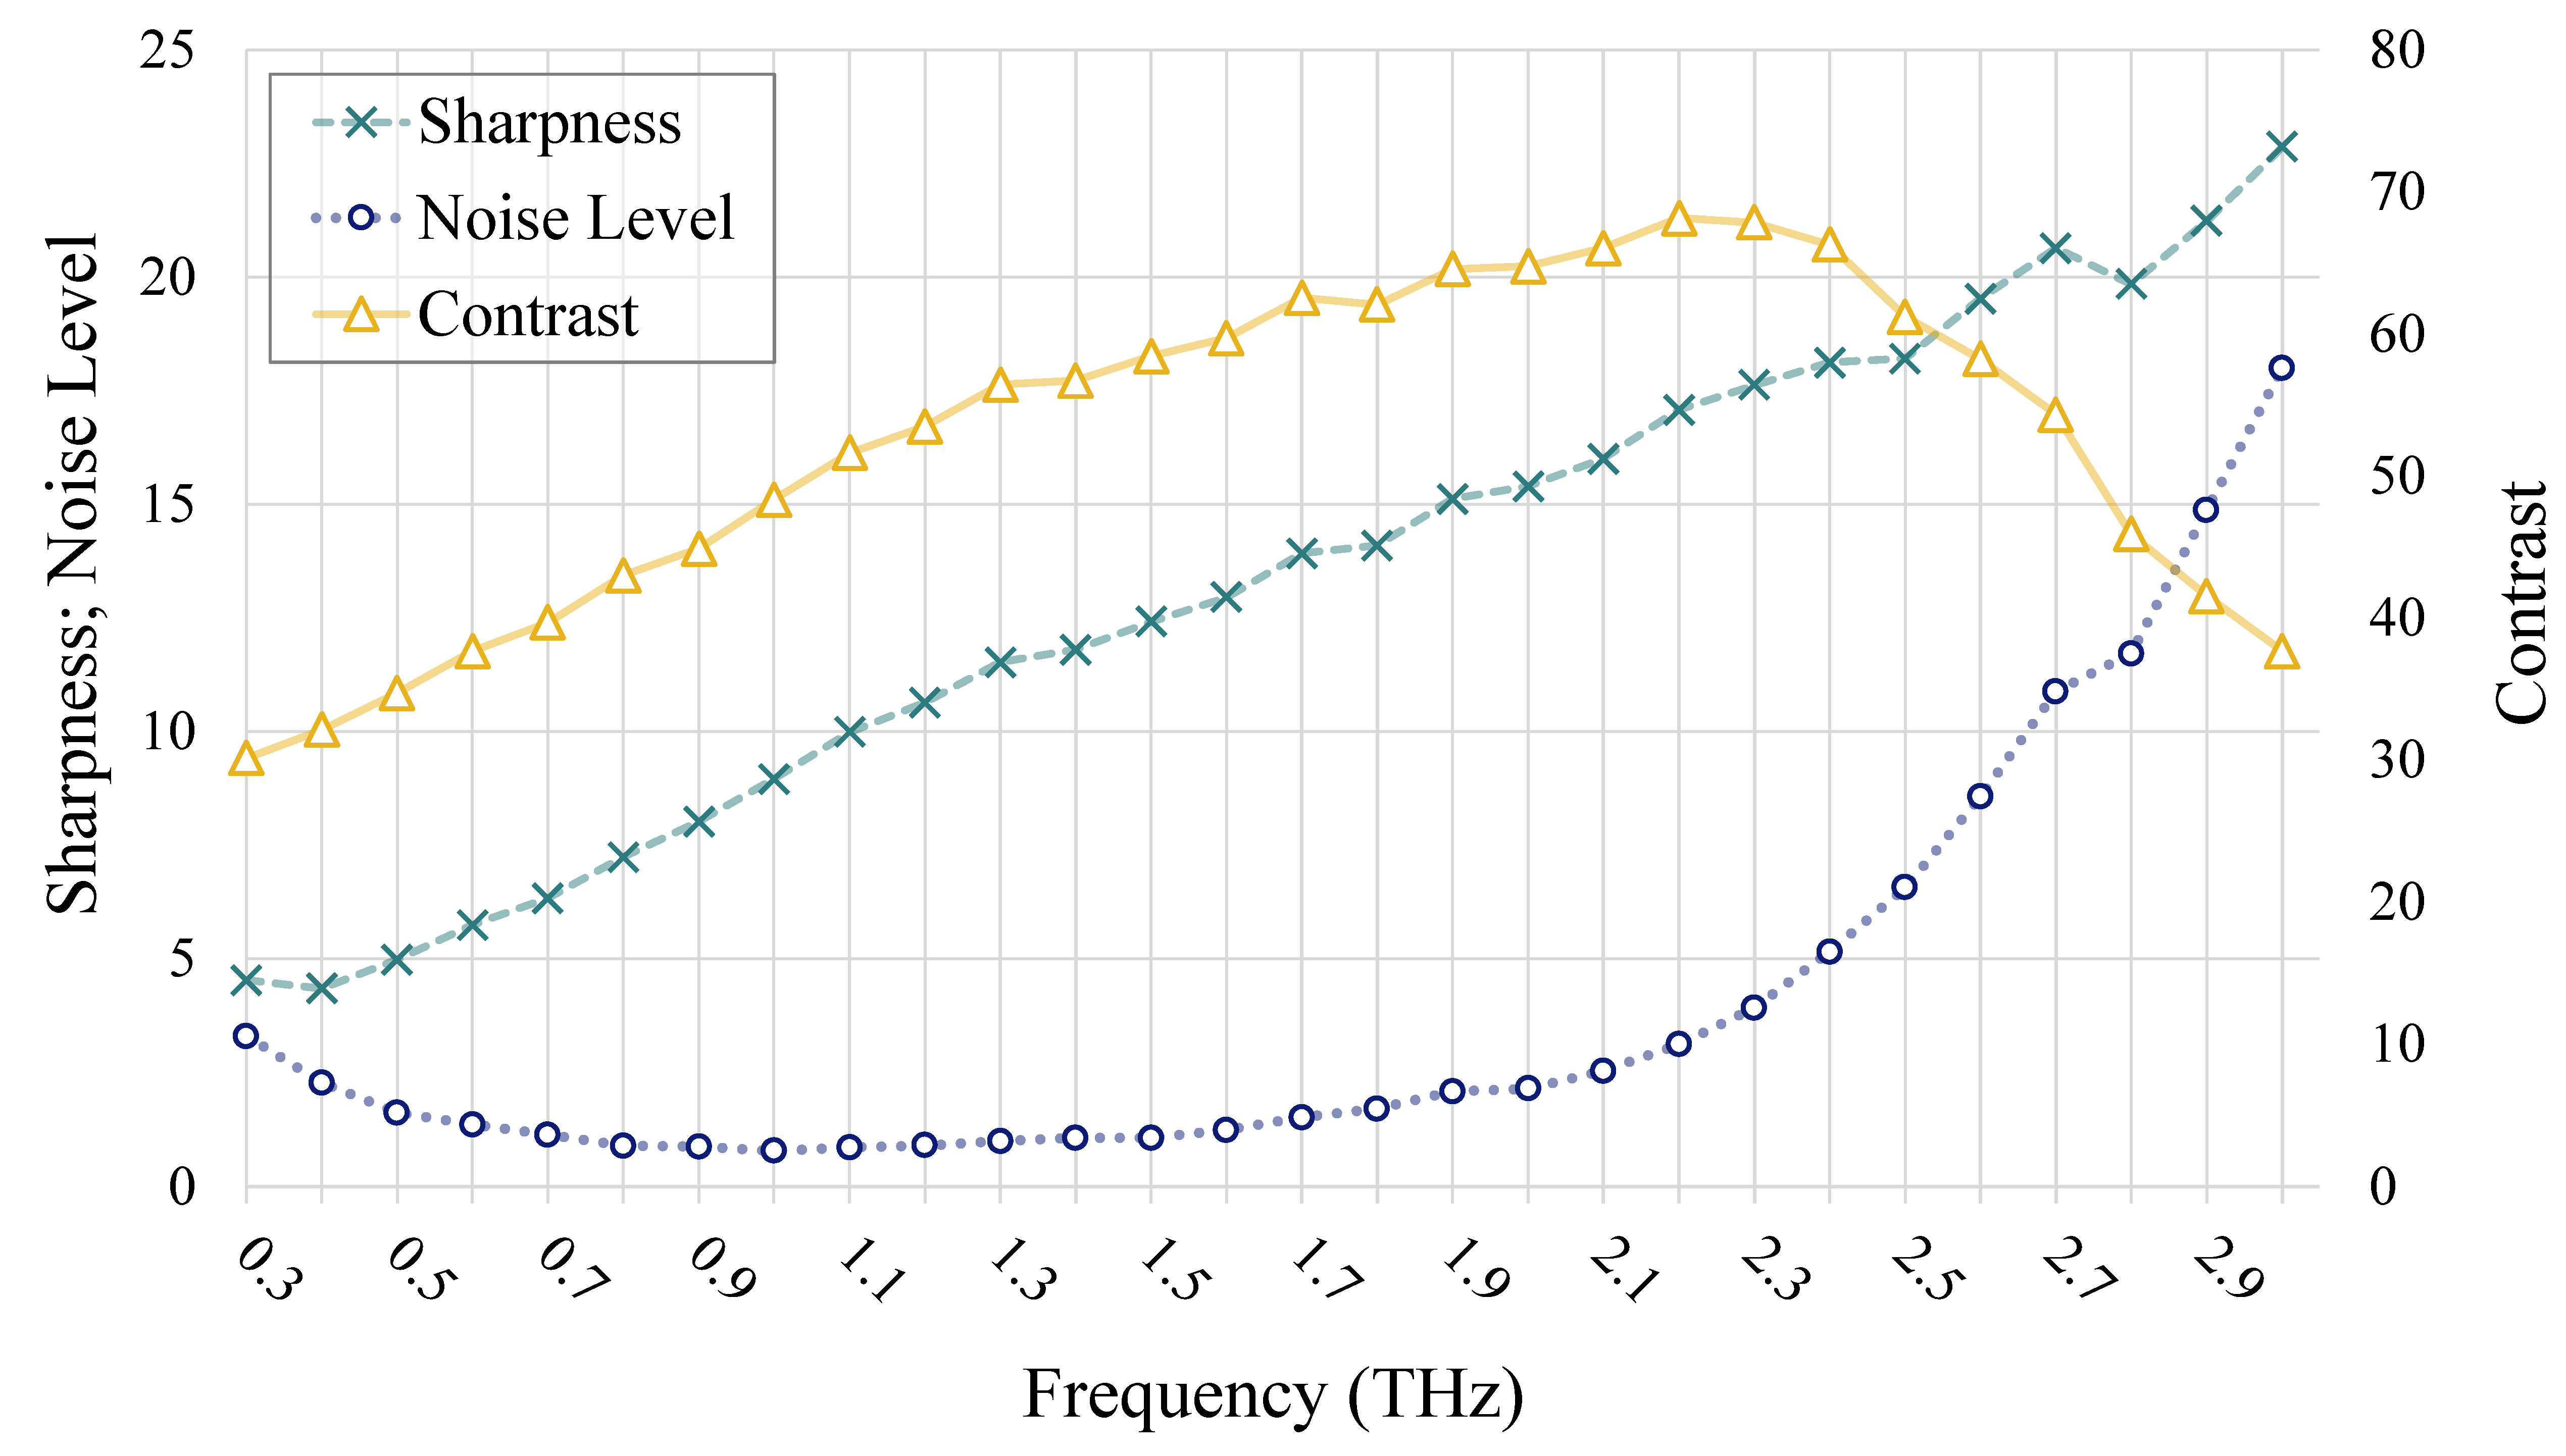
\includegraphics[width=\columnwidth]{fig/Ryu-fig2.pdf}
    \caption{Image quality assessment of the original THz SAHS images.}
    \label{fig:iqa}
\end{figure}

Conventional supervised-learning methods can be used to remove blurs in low-frequency images and noise in high-frequency images to achieve clearer images. However, applying supervised learning to THz images is challenging due to the difficulty in obtaining clean target images that directly correspond to these THz images. Hence, this study proposes a method for enhancing the quality of THz images through self-supervised learning using THz SAHS images obtained from a THz-TDS imaging system. Additionally, owing to the wavelength size and technical limitations of the imaging system, the typical image pixel resolution in THz imaging is extremely low. To overcome this, we apply image super-resolution (SR) based on self-supervised learning.

The primary objective of this study is to enhance the quality of an image obtained from a single measurement by utilizing the image. To achieve this, we propose a framework that includes a series of self-supervised image restoration methods using THz SAHS images. By performing self-supervised learning, the THz image data can be trained  without clean image targets, thereby enabling the learning of complex patterns necessary for THz image restoration.

Specifically, we train a deep learning model to learn the mapping between THz frequency bands, either from low to high frequency or vice versa. The model, which is trained to map from low to high frequency, enables blurry low-frequency images to emulate the characteristics of sharp high-frequency images. Additionally, this trained model can be applied to previously unseen images without requiring further training to render them as clear as high-frequency images. This implies that the model can overcome the diffraction limit of THz low-frequency images to yield results similar to those of high-frequency images without noise. This process of learning mapping between two frequency images can be repeated to further improve the image quality. Furthermore, using a model trained for high-to-low-frequency mapping enables noise reduction in noisy high-frequency images, although this may slightly degrade the image sharpness. Finally, we apply the zero-shot image super-resolution (ZSSR) technique, which can increase the resolution of an image by itself, to obtain visually enhanced images from a single THz SAHS image.


% 5. Main contributions %
The main contributions of this study are summarized as follows:
\begin{itemize}
\item We propose a framework that includes a series of processes to restore a single THz SAHS image obtained from a single measurement using a THz-TDS system.
\item We propose a self-supervised image restoration method based on one-to-one (O2O) mapping between frequencies, which utilizes the characteristics of a single THz SAHS image obtained via THz-TDS.
\item Our method can create images resembling high-frequency images by overcoming the diffraction limit of  low-frequency THz images and it can also reduce noise in high-frequency THz images with low SNRs.
\item The model trained using our proposed method is not limited to a specific imaging system and can be applied to all electromagnetic wave-based images.
\end{itemize}